\section{Konsistenz, UI-Konzept und Umsetzung}

\subsection{Sicherheit und geplanter Tausch}
Für die Anmeldung sind kurzlebige JWT-Zugangstoken und erneuerbare Sitzungen vorgesehen. Das Gateway prüft die Token. Jeder Dienst prüft zusätzlich die Berechtigung für die betroffene Ressource. Nutzer-IDs aus frei änderbaren Eingaben reichen dafür nicht aus. Passwörter werden mit Argon2id gehasht. Abmelden widerruft die erneuerbare Sitzung. Zugangsdaten werden geschützt auf dem Gerät abgelegt. Nur der Reverse Proxy ist öffentlich erreichbar; Datenbanken und interne Dienste bleiben im privaten Netz.

Sammlung und Tausch gehören zum Inventory Service. Beim späteren Annehmen eines Angebots werden Status und betroffene Bestände in einer Transaktion gesperrt und geprüft. Alle Mengenänderungen werden gemeinsam gespeichert oder vollständig verworfen. Bereits abgeschlossene Angebote dürfen keine zweite Änderung auslösen. Karten werden bei offenen Angeboten zunächst nicht reserviert; ihre Verfügbarkeit wird beim Annehmen erneut geprüft. \cite{postgres}

\begin{figure}[H]
\centering
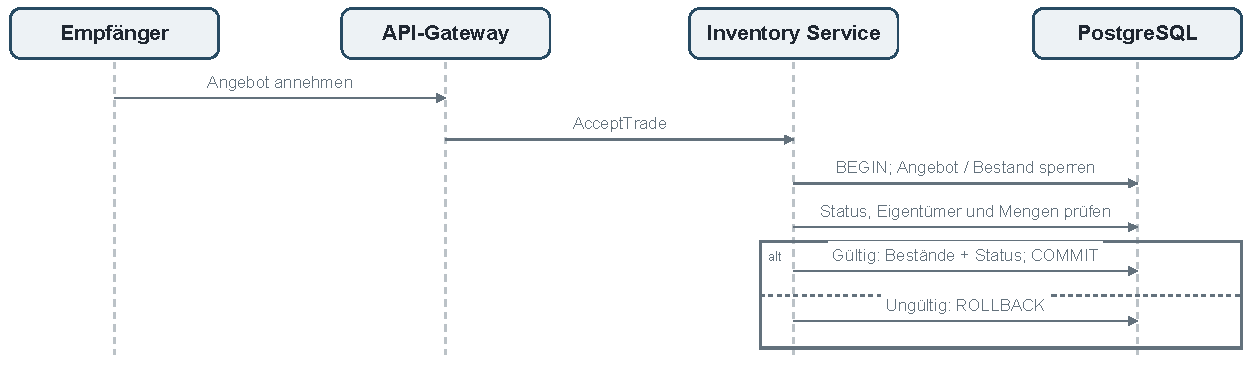
\includegraphics[width=\linewidth,height=4.7cm,keepaspectratio]{diagramme/tausch.pdf}
\caption{Annahme eines Tauschangebots im späteren Ausbau. Eigene Darstellung.}
\label{fig:tausch}
\end{figure}
\subsection{UI-Konzept und Mockup-Ablauf}
Die Zielnavigation umfasst Pokédex, Tausch, Sammlung, Freunde und Profil. Im MVP sind nur umgesetzte Bereiche aktiv. Die Sammlung bündelt Scan, manuelle Eingabe, Mengen und Wertübersicht. Kartenbilder werden stets durch Name, Set und Nummer ergänzt. Hinweise nennen eine konkrete Handlung. Das vorhandene Gestaltungskonzept orientiert sich an Apples Human Interface Guidelines; Android-Bedienmuster werden beim Geräteversuch mitgeprüft. \cite{apple}

Der Mockup-Anhang zeigt später den Weg Sammlung, Kamera, Trefferwahl, Mengenangabe und gespeicherter Eintrag. Ein zweiter Ablauf zeigt die manuelle Suche. Die Mockups stellen den geplanten Ablauf mit Beispieldaten dar. Sie sind kein Nachweis einer bereits abgeschlossenen Implementierung.

\subsection{Vorgehen und Qualitätssicherung}
Die Umsetzung beginnt mit der Anbindung des vorhandenen Erkennungsansatzes an die mobile App. Danach werden Backend-Grundlage und Anmeldung, Katalog und Preise sowie Sammlung und Scan integriert. Der MVP wird vor den sozialen Erweiterungen abgeschlossen. Schnittstellen und Abnahmekriterien werden dokumentiert. Änderungen am gemeinsamen Stand werden geprüft.

Die Abnahme prüft den Kernablauf auf Android und iOS. Dazu gehören Kameraverweigerung, falsche Treffer, Netzfehler, fehlende Preise und fremde Nutzer-IDs. Neue, bei der Entwicklung nicht genutzte Fotos dienen zur Messung von Top-1-, Top-3- und Top-5-Treffern sowie Antwortzeit und Speicherbedarf. Die bisherige Testauswahl belegt noch keine Erkennung des Gesamtkatalogs. Für den späteren Tausch werden parallele Annahmen und fehlende Karten geprüft. Der Backend-Start muss aus einem frischen Compose-Stand nachvollziehbar sein.

